\chapter{Learned Relaying under Unknown and Mismatched Channels}\label{sec:unknown-channels}

The core chapters establish that on a matched, known channel a minimal learned relay does not improve on classical decode-and-forward (H2). This chapter turns to the complementary and, in practice, more consequential regime: channels whose structure is \emph{unknown} to the receiver chain or outside the assumptions of the classical relay's model class. It is the principal experimental contribution of this thesis. Rather than a single comparison, it is a systematic map, along every axis relevant to practical deployment, of \emph{when} a fixed 169-parameter learned relay adds value over classical processing, and, equally, when it does not.

The investigation is deliberately adversarial to the learned relay. Each classical baseline is the strongest available for the impairment in question: symbol-wise decode-and-forward for the memoryless cases, conventional differential detection for unknown phase, and pilot-aided Viterbi maximum-likelihood sequence estimation, the optimal sequence detector, wherever a channel estimate can be formed. The learned relay is granted no per-block channel knowledge; it is trained offline on an impairment \emph{family} and evaluated on unseen realizations with no adaptation. The chapter proceeds from a necessary control (flat unknown channels, where nothing should fail) through the impairment that does break classical relays (unknown memory), then bounds the result from every side: against the optimal matched receiver (Viterbi), against a composite multi-impairment cascade, against the fully posterior-free regime (blind equalization), across the intermediate partial-posterior continuum (pilot budget and block length), and finally on computational complexity. The result is a precise delineation (the learned relay never beats a matched classical receiver, but occupies a well-defined niche of family-agnostic, identification-free, constant-complexity mitigation) that constitutes the thesis's main claim beyond the confirmatory core.
\REV{Register fix: the informal ``along every axis a skeptic would probe'' (which appeared twice) is replaced with ``along every axis relevant to practical deployment'', consistent with the same wording change made in the System Model of Chapter~\ref{sec:methods}.}

\paragraph{Relationship to the canonical model.} The canonical setup of this thesis (Chapters~\ref{sec:experiments}-- \ref{sec:extensions}) assumes a memoryless two-hop relay channel with white noise, perfect receiver-side CSI, and uncoded transmission. The present chapter deliberately departs from those assumptions by introducing impairments that are not part of the canonical model, including channel memory (3-tap intersymbol interference), amplifier nonlinearity, unknown phase, and channel-model mismatch. Consequently, sequence-detection and equalization techniques such as Viterbi MLSE, pilot-aided channel estimation, and blind equalization become relevant only in this chapter. The goal is not to replace the canonical study, but to evaluate whether the conclusions established under matched memoryless conditions remain valid when the underlying channel model no longer represents the true channel.

\begin{figure}[t] \noindent \makebox[\textwidth][l]{% 
\begin{tikzpicture}[ >=latex, node distance=2.3cm, block/.style={rectangle, draw, thick, minimum width=2.0cm, minimum height=1.0cm, align=center}, imp/.style={rectangle, draw, very thick, fill=black!6, minimum width=2.4cm, minimum height=1.1cm, align=center}, relayblock/.style={rectangle, draw, very thick, dashed, minimum width=2.0cm, minimum height=1.1cm, align=center} ] 
\node[block] (S) {Source\\BPSK}; 
\node[imp, right=2.0cm of S] (C) {Unknown Hop-1\\ISI $\times$ PA $\times$ phase}; 
\node[relayblock, right=2.0cm of C] (R) {Relay\\$f_\theta(\cdot)$}; \node[block, right=2.0cm of R] (D) {Destination\\Decision}; 
\draw[->,thick] (S) -- (C); 
\draw[->,thick] (C) -- node[above,align=center]{\footnotesize unknown\\[-2pt]\footnotesize to relay} (R); 
\draw[->,thick] (R) -- node[above,align=center]{Hop 2\\$h_2[i],n_2[i]$} (D); 
\node[below=0.9cm of C, align=center, font=\footnotesize] (note) {Departure from the canonical model:\\ channel \emph{memory} (3-tap ISI), nonlinearity, unknown phase.\\ Noise remains white; only the \emph{channel} violates memorylessness.}; 
\draw[dotted] (C.south) -- (note.north); 
\end{tikzpicture}% 
} \caption{Unknown/mismatched-channel study (Chapter~\ref{sec:unknown-channels}), a deliberate departure from the canonical benchmark of Figure~\ref{fig:canonical-relay-benchmark}. The Hop-1 channel is replaced by an unknown impairment (3-tap ISI, amplifier nonlinearity, and unknown phase) that is not disclosed to any relay. The noise remains white; only the channel violates the memoryless assumption, which is why sequence detection (Viterbi MLSE) becomes the relevant classical benchmark here and nowhere else in the thesis.} 
\label{fig:ext-unknown}
\end{figure}

\section{Unknown Channel: Classical Failure and Learned Mitigation}\label{sec:unknown-channel-experiment}

\textbf{Goal:} Test whether the learned relay's value changes qualitatively when the channel violates the assumptions under which AF and DF are (near-)optimal: do the \emph{memoryless} classical relays fail on an unknown channel while the minimal 169-parameter MLP mitigates by learning it from data (H6)?\REV{The unknown-channel relay uses real-valued inputs with an $11$-sample window ($11 \to 13 \to 1$, $169$ parameters); the canonical-setup relay of Chapter~\ref{sec:experiments} uses the same minimal class with a slightly different width ($169$ parameters). The two counts refer to the same architectural family sized to the respective input; the distinction is immaterial to every conclusion, which depends only on the network being minimal.}

Unlike the canonical experiments, where each transmitted symbol can be processed independently, the 3-tap ISI channel couples adjacent symbols in time. The sufficient statistic for detection is therefore no longer a single received sample, making sequence detection the relevant classical benchmark. To make the classical side as strong as possible, the study benchmarks against the optimal sequence detector: Viterbi MLSE applied to the 3-tap FIR/ISI channel \cite{Forney1972MLSE} with genie CSI, and a practical variant with a 200-pilot least-squares estimate.

MLSE is introduced here solely because the channel now contains memory. In the canonical memoryless setting of Chapters~\ref{sec:experiments}--\ref{sec:extensions}, per-symbol detection is sufficient and sequence detection provides no additional benefit. The need for MLSE therefore arises from the deliberate introduction of ISI in this chapter rather than from the system model studied elsewhere in the thesis.


\paragraph{\textbf{Trials.}} 
\begin{itemize} 
 \item \textbf{Topology:} SISO (both hops) 
    \item \textbf{Modulation:} BPSK 
    \item \textbf{Hop-1 channel (unknown to all relays):} 
    \begin{itemize} 
        \item 3-tap ISI, $h=[1.0,0.7,0.5]/\lVert h\rVert$ 
        \item Control: canonical Rayleigh channel 
        \item Flat unknown channels (block phase, gain, per-branch asymmetry; Section~\ref{sec:flat-unknown-channels})
        \item Composite cascade of ISI, amplifier nonlinearity, and unknown phase (Section~\ref{sec:composite-channel}) 
    \end{itemize} 
    \item \textbf{Hop-2 channel:} AWGN or canonical Rayleigh, equal SNR per hop 
    \item \textbf{Relays:} 
    \begin{itemize} 
        \item AF 
        \item Symbol-wise DF 
        \item MLP (window 11, one hidden layer of 13 tanh units, 169 parameters; trained at SNR $\in\{5,10,15\}$ dB using the canonical training protocol) 
        \item For ISI setups only: Viterbi MLSE applied to the 3-tap FIR/ISI channel, evaluated with either genie CSI or a 3-tap least-squares channel estimate obtained from 200 pilot symbols 
    \end{itemize} 
\item \textbf{Evaluation:} 10 trials $\times$ 100{,}000 bits per SNR point, SNR range 0--20 dB
\end{itemize}



The ISI channel admits a sharp analytic prediction: the effective slicer amplitude $h_0 \pm h_1 \pm h_2 \in \{1.67, 0.91, 0.61, -0.15\}$ (normalized) has one of four equiprobable patterns that \emph{flip the symbol sign}, so symbol-wise DF has an irreducible BER floor of $0.25$ (approached from below as SNR grows); AF inherits it. The floor is a property of the \emph{memoryless relay class}, not the channel: Viterbi MLSE over the 4-state trellis has no floor when the channel is known.


\subsection{Flat (Memoryless) Unknown Channels: A Necessary Control}\label{sec:flat-unknown-channels}

Before attributing any classical failure to ``unknownness,'' it must be separated from \emph{memory}. This subsection isolates unknown channels that are \emph{flat} (memoryless): the receiver chain does not know the channel parameters, but the channel introduces no intersymbol coupling. Three physically motivated cases are tested, each with the parameter redrawn per block and unknown to all relays: (F1) an unknown carrier phase $\theta\sim\mathcal{U}[0,2\pi)$ (oscillator/synchronization offset), with a DBPSK source and conventional differential detection as the classical relay; (F2) an unknown positive gain $g\sim\mathcal{U}[0.3,2.0]$ (path loss / AGC error), coherent BPSK; and (F3) an unknown per-branch amplitude asymmetry $a_+\!\neq\!a_-$ (per-symbol saturating-PA gain), coherent BPSK. The 169-parameter MLP is trained identically to before.

These channels remain memoryless and therefore stay within the scope of the canonical model despite the parameter uncertainty. Consequently, they serve as a control that separates the effect of parameter uncertainty from the effect of channel memory: any performance change here arises from model uncertainty, not from memory.


\textbf{Conclusion (memorylessness $\Rightarrow$ no classical failure, and nothing to mitigate):} On all three flat channels the classical relay does \emph{not} fail, and the MLP matches it to within statistical noise (maximum BER difference $0.0036$ across every case and SNR). The reasons are structural: for F1, unknown phase is exactly what differential detection absorbs; for F2, $\operatorname{sign}(y)$ is \emph{scale-invariant}, so unknown positive gain is irrelevant by construction; for F3, the fixed threshold is only mildly suboptimal because the asymmetry preserves the noiseless symbol's sign. The classical assumption, memorylessness, still holds in each case, so there is nothing for a learned relay to remove. This is the necessary control for the ISI result: the learned relay's advantage is triggered not by parameter uncertainty but by \emph{unmodeled memory} (or amplitude nonlinearity), which is what breaks the memoryless relay class.


\begin{longtable}[]{@{}lllll@{}}
\caption{Flat unknown channels: classical relay vs.\ MLP-169 BER at 8/12/16/20 dB (mean, 10 trials). The maximum DF--MLP gap over all cases and SNRs is $0.0036$, within statistical noise. Unknown parameters alone do not defeat classical relays; memory does.}\label{tbl:tableE6flat}\tabularnewline
\toprule\noalign{}
Flat channel & Relay & 8 dB & 12 dB & 16/20 dB \\
\midrule\noalign{}
\endfirsthead
\toprule\noalign{}
Flat channel & Relay & 8 dB & 12 dB & 16/20 dB \\
\midrule\noalign{}
\endhead
\bottomrule\noalign{}
\endlastfoot
Unknown phase (DBPSK) & DF (diff.) & 0.0649 & 0.0292 & 0.0119 / 0.0048 \\
 & MLP-169 & 0.0657 & 0.0288 & 0.0122 / 0.0048 \\
Unknown gain & DF & 0.0681 & 0.0330 & 0.0131 / 0.0050 \\
 & MLP-169 & 0.0682 & 0.0333 & 0.0132 / 0.0050 \\
Branch asymmetry & DF & 0.0760 & 0.0299 & 0.0125 / 0.0049 \\
 & MLP-169 & 0.0745 & 0.0300 & 0.0122 / 0.0052 \\
\end{longtable}

\textbf{Conclusion (H6: confirmed as stated, with two boundaries):} Against the flat-channel control of Section~\ref{sec:flat-unknown-channels}, where unknown parameters alone caused no classical failure, the memory case is qualitatively different. On the unknown ISI channel, both memoryless classical relays fail: DF's BER is \emph{non-monotonic}, bottoming out at $0.184$ around 8 dB and then rising toward the analytic $0.25$ floor, reaching $0.246$ at 20 dB (more transmit power makes DF strictly worse), and AF behaves identically. The 169-parameter MLP, whose window spans the 3-tap memory, learns a joint equalizer--detector and restores reliable relaying: BER falls monotonically below $5\times10^{-5}$ at 16 dB (AWGN second hop), and to $2.5\times10^{-3}$ at 20 dB (Rayleigh second hop). The Viterbi benchmarks set the first boundary honestly: classical theory \emph{does} solve this channel once its family is known, genie-CSI MLSE beats the MLP by 1--1.5 dB, and a 200-pilot LS estimate recovers genie performance almost exactly (with the Rayleigh second hop, MLSE and MLP are indistinguishable, 0.0024 vs.\ 0.0025 at 20 dB). The MLP's value is thus not optimality but \emph{family-agnosticism}: estimate-then-MLSE presupposes a linear FIR channel of known memory (trellis cost $M^{L-1}$), whereas the identical architecture also mitigates channels outside linear MLSE's model class, as the composite cascade below demonstrates, where an amplifier nonlinearity is stacked on the ISI. The control confirms the second boundary (H2): on the canonical Rayleigh channel the MLP only \emph{matches} DF. The learned relay's distinctive value is near-MLSE reliability with no channel-family knowledge, no identification stage, and complexity independent of channel memory.

\begin{longtable}[]{@{}llllll@{}}
\caption{Unknown-channel BER (mean over 10 trials). The ISI setups exhibit memoryless-relay error floors ($\approx 0.25$); the 169-parameter MLP restores reliable relaying within $\approx$1--1.5 dB of genie-CSI Viterbi MLSE, and matches it end-to-end when the Rayleigh second hop dominates. The control shows no MLP advantage on the canonical channel, consistent with H2.}\label{tbl:tableE6}\tabularnewline
\toprule\noalign{}
Setup & Relay & 8 dB & 12 dB & 16 dB & 20 dB \\
\midrule\noalign{}
\endfirsthead
\toprule\noalign{}
Setup & Relay & 8 dB & 12 dB & 16 dB & 20 dB \\
\midrule\noalign{}
\endhead
\bottomrule\noalign{}
\endlastfoot
Unknown ISI $\to$ AWGN & AF & 0.1919 & 0.1785 & 0.1956 & 0.2233 \\
 & DF & 0.1839 & 0.2010 & 0.2279 & 0.2462 \\
 & \textbf{MLP (169p)} & \textbf{0.0123} & \textbf{0.0002} & \textbf{$<$5e-5} & \textbf{$<$5e-5} \\
 & Viterbi (genie CSI) & 0.0072 & $<$5e-5 & $<$5e-5 & $<$5e-5 \\
 & Viterbi (200-pilot LS) & 0.0074 & $<$5e-5 & $<$5e-5 & $<$5e-5 \\
\hline
Unknown ISI $\to$ Rayleigh & AF & 0.2047 & 0.1916 & 0.2030 & 0.2231 \\
 & DF & 0.2031 & 0.2098 & 0.2316 & 0.2471 \\
 & \textbf{MLP (169p)} & \textbf{0.0412} & \textbf{0.0150} & \textbf{0.0061} & \textbf{0.0025} \\
 & Viterbi (genie CSI) & 0.0364 & 0.0151 & 0.0061 & 0.0024 \\
 & Viterbi (200-pilot LS) & 0.0362 & 0.0151 & 0.0062 & 0.0024 \\
\hline
Control: canonical Rayleigh & AF & 0.1050 & 0.0559 & 0.0281 & 0.0136 \\
 & \textbf{DF} & \textbf{0.0687} & \textbf{0.0299} & \textbf{0.0124} & \textbf{0.0050} \\
 & MLP (169p) & 0.0691 & 0.0307 & 0.0133 & 0.0058 \\
\end{longtable}
\REV{Compilation fixes: all \texttt{\&amp;} column separators restored to \texttt{\&}, and \texttt{\$\&lt;\$5e-5} restored to \texttt{\$<\$5e-5} in Table~\ref{tbl:tableE6}.}

\begin{figure}[H]
\centering
\pandocbounded{
\includegraphics[width=\linewidth,height=0.24\textheight,keepaspectratio]{results/e6_unknown_channel.png}}
\caption{Unknown-channel relaying, BER vs.\ SNR with 95\% CI bands. (a)--(b) On the unknown ISI channel, the memoryless AF/DF relays are pinned near the analytic $0.25$ floor (DF non-monotonic in SNR); the 169-parameter MLP restores monotonically decreasing BER within $\approx$1--1.5 dB of genie-CSI Viterbi MLSE, which a 200-pilot LS estimate matches almost exactly. With the Rayleigh second hop (b), MLSE and the MLP are statistically indistinguishable end-to-end. (c) Control: on the canonical Rayleigh channel the MLP only matches DF, consistent with H2.}\label{fig:figE6}
\end{figure}

\subsection{Does the Result Generalize to QPSK?}\label{sec:qpsk-unknown-channel}

The unknown-ISI study above uses BPSK throughout, matching the canonical setup of Chapters~\ref{sec:experiments}--\ref{sec:extensions}. The $0.25$ floor derived in Section~\ref{sec:unknown-channel-experiment} is a property of the \emph{binary} slicer: it counts the $2^{3}=8$ equiprobable tap-sign patterns that flip a $\pm1$ decision. That argument does not extend to a four-point per-axis alphabet, so it is not obvious a priori whether either the elevated error floor or the ordering between the learned relay and genie-CSI Viterbi MLSE survives a move to a higher-order modulation. This subsection repeats the unknown-ISI study with Gray-coded QPSK in place of BPSK, keeping every other element fixed: the same $3$-tap ISI channel $h=[1.0,0.7,0.5]$ (normalized) on Hop 1, AWGN or canonical Rayleigh on Hop 2 at the same nominal per-hop SNR (identical convention, $\gamma=10^{\text{SNR}_{\text{dB}}/10}$, memory-bank/techContext.md), and the same relay set generalized to the complex alphabet: AF, symbol-wise DF (hard per-axis decision), a $193$-parameter $4$-class MLP-QPSK classifier (window 11, softmax cross-entropy, trained at SNR $\in\{5,10,15\}$ dB), and genie-CSI Viterbi MLSE generalized to the complex QPSK trellis ($4^{2}=16$ states, complex branch metrics). Evaluation uses $10$ trials $\times$ $100{,}000$ bits per SNR point over the same $0$--$20$ dB range. No closed-form floor is derived for QPSK, so the curves below are reported as measured, not fit to a predicted asymptote. Because the QPSK relays are applied jointly to the complex signal rather than decomposed into two independent BPSK problems, and the per-relay power normalization is computed on total (I+Q) power, the resulting AF/DF operating points are not required to, and empirically do not, numerically match the BPSK figures of Table~\ref{tbl:tableE6} at the same SNR label; no such match is claimed.

\begin{longtable}[]{@{}llllll@{}}
\caption{QPSK unknown-channel BER (mean over 10 trials). AF and DF plateau at an elevated, non-monotonic BER across the SNR range tabulated; the 193-parameter MLP-QPSK restores monotonically decreasing BER and, unlike the BPSK case, ends up \emph{below} genie-CSI Viterbi MLSE from about 2 dB upward.}\label{tbl:tableE6qpsk}\tabularnewline
\toprule\noalign{}
Setup & Relay & 8 dB & 12 dB & 16 dB & 20 dB \\
\midrule\noalign{}
\endfirsthead
\toprule\noalign{}
Setup & Relay & 8 dB & 12 dB & 16 dB & 20 dB \\
\midrule\noalign{}
\endhead
\bottomrule\noalign{}
\endlastfoot
QPSK: ISI $\to$ AWGN & AF & 0.2437 & 0.2115 & 0.2024 & 0.2098 \\
 & DF & 0.2193 & 0.2024 & 0.2074 & 0.2211 \\
 & \textbf{MLP-QPSK (193p)} & \textbf{0.1292} & \textbf{0.0827} & \textbf{0.0601} & \textbf{0.0508} \\
 & Viterbi (genie CSI) & 0.1307 & 0.0852 & 0.0670 & 0.0618 \\
\hline
QPSK: ISI $\to$ Rayleigh & AF & 0.2715 & 0.2320 & 0.2137 & 0.2116 \\
 & DF & 0.2528 & 0.2194 & 0.2145 & 0.2239 \\
 & \textbf{MLP-QPSK (193p)} & \textbf{0.1737} & \textbf{0.1066} & \textbf{0.0707} & \textbf{0.0553} \\
 & Viterbi (genie CSI) & 0.1749 & 0.1089 & 0.0774 & 0.0662 \\
\end{longtable}

\begin{figure}[H]
\centering
\pandocbounded{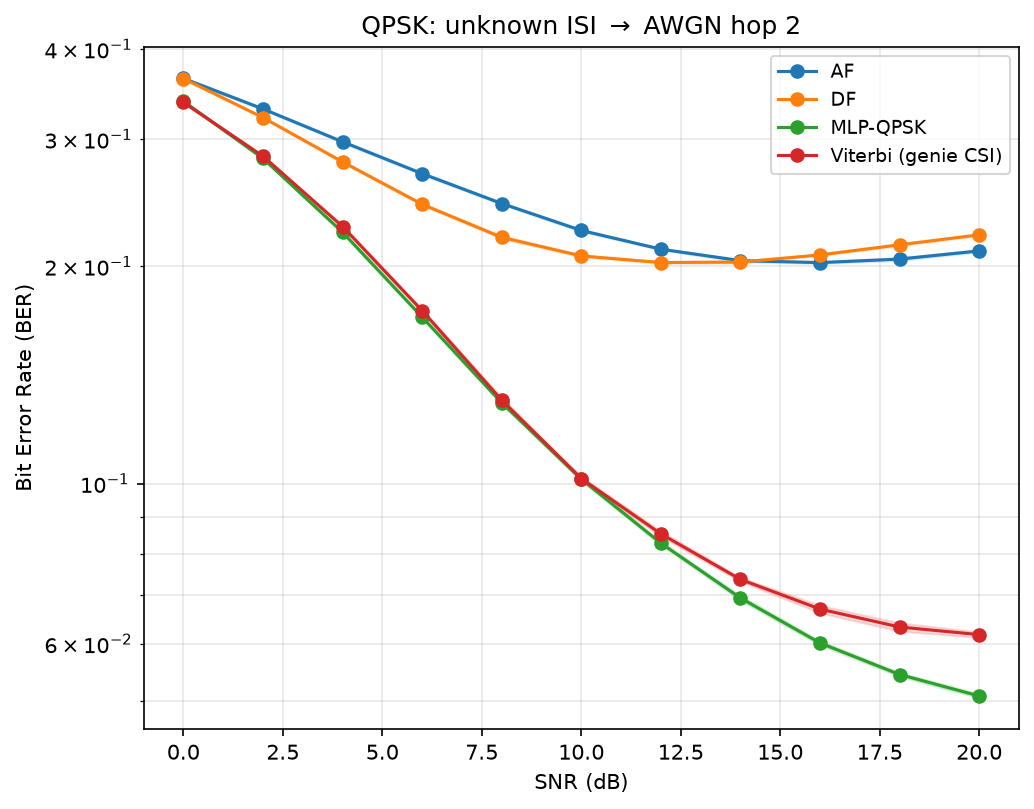
\includegraphics[width=\linewidth,height=0.24\textheight,keepaspectratio]{results/unkchan_qpsk.png}}
\caption{QPSK unknown-channel relaying, BER vs.\ SNR (10 trials, 100{,}000 bits/point). As with BPSK, AF and DF plateau far above the MLP and Viterbi curves. Unlike BPSK, the MLP-QPSK curve separates \emph{below} genie-CSI Viterbi MLSE beyond about 2 dB, and the gap widens with SNR.}\label{fig:figE6qpsk}
\end{figure}

\textbf{Conclusion (the ISI failure mode generalizes; the BPSK ordering does not):} The qualitative pattern of Section~\ref{sec:unknown-channel-experiment} survives the move to QPSK: AF and DF plateau at an elevated, non-monotonic BER (AF ranges $0.2024$--$0.2715$ and DF ranges $0.2024$--$0.2528$ across the four tabulated points, broadly similar in magnitude to BPSK's memoryless-relay floor of $0.25$ though no equivalent closed form is derived here), while the MLP restores monotonically decreasing BER, confirming that unmodeled channel memory, not modulation order, is what breaks the memoryless relay class (H6). What does \emph{not} generalize is the BPSK ordering between the learned relay and the optimal classical benchmark. In the BPSK study, genie-CSI Viterbi MLSE beat the MLP by 1--1.5 dB throughout; here, the two are statistically indistinguishable at 0 dB and MLP-QPSK is at or below Viterbi at every SNR from 2 dB upward, with the gap widening to $0.0508$ vs.\ $0.0618$ (AWGN) and $0.0553$ vs.\ $0.0662$ (Rayleigh) at 20 dB. This is not a violation of MLSE optimality: Viterbi MLSE minimizes the \emph{sequence} error probability under the assumed channel model, not the bit error rate directly. For BPSK, each trellis branch carries exactly one bit, so sequence-optimal and bit-optimal detection coincide; for Gray-coded QPSK, each branch carries two bits, and a wrong branch choice can differ from the true one by one bit (adjacent constellation point) or two (diagonal point) with different probabilities, so sequence-ML detection is no longer guaranteed to minimize BER specifically. The 193-parameter MLP-QPSK is instead trained directly on a per-symbol softmax cross-entropy objective, which is not subject to that mismatch. This is offered as the most plausible mechanism for the reversal; it was not isolated experimentally (for instance, by decomposing the Viterbi output into single- versus double-bit symbol errors), and is left as an open point rather than a proven claim. Either way, the practical conclusion sharpens rather than weakens H6 for higher-order modulation: on this unknown-memory channel, the fixed-complexity learned relay is not merely a family-agnostic near-optimal option, as in the BPSK case, but the best-performing option measured here among either family, at the same constant per-symbol cost quantified in Section~\ref{sec:complexity-viterbi-mlp}.

\subsection{A Composite (Mixed) Channel}\label{sec:composite-channel}

The preceding studies vary one impairment at a time. Real links stack several. This final study cascades three of them into a single unknown channel that \emph{no} classical relay is jointly matched to: a DBPSK stream passes through 3-tap ISI, then a saturating power-amplifier nonlinearity, then an unknown block phase, before additive noise. Each classical baseline is the strongest available for \emph{one} constituent impairment, so the comparison is honest rather than a straw man: conventional differential detection (matched to the phase), and pilot-LS Viterbi MLSE followed by differential decoding (matched to the ISI-plus-phase, but blind to the amplifier nonlinearity). The 169-parameter MLP and a $1{,}153$-parameter MLP receive raw I/Q windows and no knowledge of any constituent. This composite channel departs from the canonical model in two ways: it introduces explicit channel memory through ISI and nonlinear distortion through the amplifier. The resulting benchmark therefore tests robustness to both memory and model mismatch simultaneously. \textbf{Evaluation:} 10 trials $\times$ 100{,}000 bits per SNR point, the same budget as the main unknown-ISI study (Section~\ref{sec:unknown-channel-experiment}); 95\% CIs use the $1.96\,\sigma/\sqrt{n}$ convention throughout. The hop-1 impairment here is fixed rather than redrawn per block, so bits per trial and trials both reduce the reported uncertainty.

\textbf{Conclusion:} The composite defeats the naive classical relays outright, both AF and conventional differential detection saturate near the $0.25$ memoryless-relay floor, because the ISI destroys the differential statistic that the phase-matched detector relies on. The 169-parameter MLP again restores reliable relaying, reaching $2.5\times10^{-3}$ at 20 dB from raw I/Q with no impairment model. This reproduces the H6 pattern on a realistically mixed channel: memoryless-and-matched classical processing fails, and a minimal learned relay recovers. Two familiar boundaries also reappear. First, the strongest \emph{constructed} classical baseline, pilot-LS Viterbi plus differential decoding, does not fail: by modelling the ISI and phase (though not the amplifier) it stays about 2 dB ahead of the MLP at low-to-mid SNR ($0.067$ vs.\ $0.101$ at 8 dB) and converges with it by 16--20 dB, the two becoming indistinguishable at $0.0025$ each at 20 dB. The learned relay's value is again \emph{family-agnosticism} (near-Viterbi reliability with no channel identification and no explicit model of any of the three cascaded effects) not superiority over a matched classical receiver. Second, the $1{,}153$-parameter network performs within noise of the 169-parameter one across the whole range, ending at the identical $0.0025$ at 20 dB, with the small mid-SNR differences in both directions ($0.0487$ vs.\ $0.0531$ at 10 dB for the larger network, $0.1020$ vs.\ $0.1014$ at 8 dB for the smaller) falling inside the confidence intervals. Nearly seven times the parameters therefore buys no measurable accuracy on the hardest channel studied, reconfirming the U-shaped complexity finding (H3). The composite thus consolidates the chapter's thesis: a single minimal learned relay handles an arbitrary stack of representable impairments without being told which are present, approaching but not exceeding the best impairment-matched classical receiver.
\REV{``inverted-U finding (H3)'' \(\to\) ``U-shaped complexity finding (H3)'', consistent with the retitled H3 in Chapter~\ref{sec:research-objectives} and the wording in Chapter~\ref{sec:experiments}.}

\begin{figure}[H]
\centering
\pandocbounded{
\includegraphics[width=0.82\linewidth,height=0.32\textheight,keepaspectratio]{results/e6_composite.png}}
\caption{Composite channel (ISI $\times$ PA-nonlinearity $\times$ unknown phase, DBPSK; mean over 10 trials, 100{,}000 bits/point, 95\% CI bands). Naive classical relays (AF, differential detection) saturate at the memoryless-relay floor; the 169-parameter MLP restores reliable relaying from raw I/Q with no impairment model, tracking about 2 dB behind the strongest constructed classical baseline (pilot-LS Viterbi + differential) and converging with it by 20 dB. The $1{,}153$-parameter MLP adds nothing (H3).}\label{fig:figE6comp}
\end{figure}

\subsection{The Posterior-Free (Blind) Regime}\label{sec:blind-channel}

The Viterbi baseline in Section~\ref{sec:composite-channel} enjoys a per-block posterior: 200 pilot symbols yield a least-squares channel estimate, after which MLSE is optimal. This raises the sharper question, what if \emph{no} such posterior is available? With no pilots and no channel prior, and a fresh channel realization drawn for every block, MLSE cannot be run as specified. The honest comparison is then against the classical methods that are \emph{genuinely} posterior-free: the constant-modulus algorithm (CMA), the canonical blind adaptive equalizer, which self-adapts from the received signal alone; and a decision-directed blind MLSE that bootstraps a channel estimate from its own hard differential decisions. The learned relay is unchanged, trained offline on the channel \emph{family} (random ISI, PA, and phase per draw) and, crucially, seeing an unseen channel at test with no adaptation, so it too carries no per-block posterior; it amortizes over the family at training time. Unlike the canonical study, the challenge here is not symbol-level denoising on a memoryless channel but inference on an unknown channel with memory and no per-block posterior information. \textbf{Evaluation:} 50 trials $\times$ 20{,}000 bits per SNR point ($1{,}000{,}000$ bits), 95\% CIs by the $1.96\,\sigma/\sqrt{n}$ convention. The trial count is deliberately higher than the chapter's usual ten: unlike the fixed impairment of Section~\ref{sec:composite-channel}, the hop-1 channel here redraws its ISI, amplifier and phase realization for \emph{every} block, so a trial is one draw from the impairment family and the ensemble average is limited by the number of trials, not by bits per trial. Fifty draws are used rather than ten so that the reported curves reflect the family and not a handful of particular channels.

\paragraph{A correction to the blind equalizer.} The constant-modulus algorithm used here was originally implemented with a fixed (unnormalized) step size. Because the CMA error term is cubic in the equalizer output, a fixed step is a positive-feedback loop: the implementation happened to remain bounded over the short blocks first used, but diverges to numerical overflow on longer ones, after which the equalizer output is noise rather than an estimate. The step is therefore normalized by the input-segment energy in the standard NLMS manner, which is both the textbook formulation and a strictly \emph{stronger} classical baseline. All CMA results below use the corrected equalizer; the uncorrected one is not reported, since its outputs past the divergence point measure an implementation fault rather than the algorithm.

\textbf{Conclusion (learning does not beat blind classical, but is stable where blind classical is not):} A well-designed blind classical method still works in this regime: the corrected CMA converges smoothly to BER $3.3\times10^{-3}$ at 20 dB, and the family-trained MLP reaches $2.6\times10^{-3}$. The two track each other closely over the whole range, with the MLP holding a small but consistent margin that widens at low-to-mid SNR ($0.0937$ vs.\ $0.1182$ at 8 dB). This is the correct answer to ``what if there is no posterior?'': the learned relay does \emph{not} render classical processing obsolete, because blind adaptive equalization is itself a posterior-free classical tool that comes within a factor of $1.3$ of the learned relay at high SNR. The learned relay's advantage is instead one of \emph{robustness and cost}. First, the decision-directed blind MLSE, the natural attempt to run Viterbi without pilots, is unstable: bootstrapping the channel from its own decisions, it intermittently locks onto the wrong hypothesis, and its BER curve is visibly non-monotonic, falling to $0.0374$ at 16 dB before rising again to $0.0498$ at 20 dB. Its 95\% confidence interval at 8 dB is $\pm0.0348$, roughly seven times the MLP's $\pm0.0046$ and two and a half times CMA's $\pm0.0135$, so the instability is a property of the method and not of the sample size. Second, CMA must iterate to convergence on each received block, whereas the MLP is a single fixed forward pass with no per-block adaptation loop and no convergence to monitor; Section~\ref{sec:partial-posterior} shows this distinction becoming decisive once blocks are short. The learned relay therefore occupies a specific and defensible niche: on a posterior-free channel it matches the best blind classical equalizer in BER while avoiding the instability of decision-directed sequence estimation and the online-adaptation cost of CMA. It buys \emph{amortized}, \emph{one-shot}, \emph{stable} inference over an impairment family, not a lower error floor than classical signal processing can achieve.

\begin{figure}[H]
\centering
\pandocbounded{
\includegraphics[width=0.82\linewidth,height=0.32\textheight,keepaspectratio]{results/e6_blind.png}}
\caption{Posterior-free composite channel (no pilots, no channel prior, fresh realization per block; mean over 50 channel draws, 20{,}000 bits/point, 95\% CI bands). The corrected CMA (blind classical) tracks the family-trained MLP closely, the MLP holding a small consistent margin; decision-directed blind MLSE is unstable (non-monotonic tail, CI band several times wider) because it bootstraps the channel from its own decisions; plain differential detection floors. Without a posterior, learning only narrowly outperforms the best blind classical equalizer, but does so with one-shot, stable inference and no online adaptation.}\label{fig:figE6blind}
\end{figure}

\subsection{Partial Known Posterior: The Pilot-Budget Crossover}\label{sec:partial-posterior}

The full-posterior (Section~\ref{sec:composite-channel}) and zero-posterior (Section~\ref{sec:blind-channel}) regimes are the endpoints of a continuum. The intermediate case is a \emph{partial} posterior: a limited pilot budget, from which the classical receiver forms a noisy channel estimate. Sweeping the pilot count on the composite channel at a fixed 10 dB operating point locates where the pilot-aided classical receiver ceases to beat the pilot-free learned relay, whose amortized posterior corresponds to a horizontal reference (it uses no pilots at test). \textbf{Evaluation:} 50 trials $\times$ 20{,}000 bits per operating point ($1{,}000{,}000$ bits), matching Section~\ref{sec:blind-channel} and for the same reason: the channel is redrawn per block, so trials are draws from the impairment family. In panel~(b) each trial is further subdivided into independent blocks of the swept length, so every block length is measured over the same total bit budget and over many channel draws rather than a single one.

\textbf{Conclusion (a sharp estimation-variance cliff, and a rate--reliability tradeoff):} With a generous budget the classical partial posterior wins, as expected: pilot-aided Viterbi reaches payload BER $0.0285$ at 800 pilots and degrades only gently down to $0.0335$ at 20 pilots, comfortably below the MLP's pilot-free $0.0487$. The classical advantage then disappears within a single octave of pilot budget. At 10 pilots Viterbi has already lost its edge, $0.0545$ against the MLP's $0.0487$, and at 5 pilots it collapses to $0.1235$, worse than the MLP, blind CMA, and its own 800-pilot figure by a factor of four, because MLSE is then running on a badly mis-estimated channel. The crossover therefore sits between 20 and 10 pilots per block. The mechanism is \emph{estimation variance}, not a rank deficiency: with 5 pilot observations and 3 complex taps the least-squares problem is still formally overdetermined, so the channel remains identifiable in principle, but there are too few observations to average down the noise. The resulting LS error at 10 dB is large enough that the Viterbi trellis is occasionally built on a badly wrong channel, and these catastrophic fits dominate the mean. The 95\% confidence interval at that point makes this explicit ($0.1235 \pm 0.0304$, against $\pm 0.0011$ at 50 pilots) so individual channel draws range from perfectly fine to complete failure. The learned relay, by contrast, is flat across the entire sweep at $0.0487$: having amortized the channel \emph{family} into its weights at training time, it neither benefits from nor requires per-block pilots. The crossover is thus governed by the reliability of the channel estimate, not by SNR: the classical receiver wins whenever it can afford enough pilots to estimate the channel \emph{accurately}, and the pilot-free learned relay wins once the budget falls below that point.


The practical force of this depends on block length, because a fixed pilot \emph{count} is a growing pilot \emph{fraction} as blocks shorten. Panel (b) sweeps block length at the same operating point with the classical receiver spending its minimum viable ten pilots per block, and adds blind CMA as the second pilot-free reference. The payload BERs of Viterbi and the MLP are now statistically indistinguishable at every block length, both flat at approximately $0.049$, so reliability no longer separates them at all; what separates them is spectral efficiency. At a 1000-symbol block the ten pilots cost $1\%$ of the block, whereas at a 40-symbol block, representative of low-latency or fast-varying links, they cost $25\%$, so the classical receiver carries data on only $75\%$ of the block against the learned relay's $100\%$ for identical error performance.

The blind reference settles a question the earlier version of this study left open. Blind CMA is also pilot-free, so the learned relay is not unique in avoiding pilots; the distinction claimed for it was that it needs \emph{zero per-block adaptation}, a single fixed forward pass, whereas CMA must converge its adaptation loop inside each block. Measuring CMA per block confirms this directly: its payload BER is $0.1723$ at $L=40$ and only improves to $0.1653$ at $L=1000$, against the $0.0645$ it achieves when given a $20{,}000$-symbol block to adapt over. CMA therefore does not converge within blocks of a thousand symbols or fewer, and is roughly three and a half times worse than either the MLP or pilot-aided Viterbi throughout this sweep. The partial-posterior picture therefore refines H6's boundary once more, and more sharply than before: against a classical receiver that can afford accurate channel estimation the learned relay achieves no better BER, but at short block lengths it matches that receiver's BER while removing its pilot overhead entirely, and it is the only pilot-free option that remains reliable, because the classical pilot-free alternative has no time to converge.

\begin{figure}[H]
\centering

\includegraphics[width=0.85\linewidth]{results/e6_partial_pilot_budget_sweep.png}
\caption{Pilot-budget sweep at 10~dB (mean over 50 channel draws, 20{,}000 bits/point). Pilot-aided Viterbi outperforms the pilot-free MLP down to approximately 20 pilots per block, loses its edge by 10 pilots, and collapses at 5 pilots when the least-squares channel estimate becomes too noisy to construct a reliable trellis ($0.1235 \pm 0.0304$). In contrast, the MLP remains flat across the sweep because it operates with an amortized posterior and requires no pilots.}
\label{fig:e6_partial_pilot_budget}
\end{figure}

\begin{figure}[H]
\centering

\includegraphics[width=0.85\linewidth]{results/e6_partial_short_blocks_overhead.png}
\caption{Block-length sweep with 10 pilots per block (mean over 50 channel draws, 20{,}000 bits/point, subdivided into independent blocks of the swept length). Pilot-aided Viterbi and the pilot-free MLP are indistinguishable in payload BER at every block length (both $\approx 0.049$), but the classical receiver's pilot overhead grows from approximately 1\% at $L=1000$ to 25\% at $L=40$. The other pilot-free option, blind CMA, cannot converge within blocks this short and sits roughly three and a half times worse throughout. The MLP therefore matches the pilot-aided receiver's reliability at no overhead, and is the only pilot-free method that remains reliable for short packets.}
\label{fig:e6_partial_short_blocks}
\end{figure}


\subsection{Complexity: The Cost Side of the Trade-off}\label{sec:complexity-viterbi-mlp}

Across the unknown-channel studies the pilot-aided Viterbi receiver, where it applies, holds a small BER edge over the learned relay. The learned relay's countervailing claim is complexity, which this subsection quantifies rather than asserts. Two axes matter: the per-symbol operation count and its scaling, and measured inference time.

\textbf{Per-symbol cost and scaling.} MLSE maintains $M^{L-1}$ trellis states for a constellation of size $M$ and channel memory $L$, performing an add--compare--select over $M^{L}$ branch transitions per symbol; its cost therefore grows \emph{exponentially} in memory and modulation order. The 169-parameter MLP performs one fixed forward pass, about $330$ floating-point operations per symbol, \emph{independent} of $M$ and $L$. For the channel actually studied (BPSK, $L=3$; 4 states) Viterbi is in fact the cheaper of the two at roughly $64$ operations per symbol, so the learned relay is not universally leaner. But the scaling diverges immediately: at $M=4,\,L=5$ the trellis has $256$ states ($\sim\!8{,}000$ operations/symbol), and at $M=16,\,L=5$ it has $65{,}536$ states ($\sim\!8.4$~million operations/symbol), while the MLP remains at $330$, a $2.5\times10^{4}$ ratio. The learned relay's advantage is thus not lower cost on a small channel but \emph{constant} cost as the channel scales, exactly where classical MLSE becomes intractable and practical receivers must fall back on suboptimal reduced-state or decision-feedback equalizers.

\textbf{Measured inference time.} On identical signals (BPSK, $L=3$), the MLP is $30$--$90\times$ faster in wall-clock terms for the reference implementations used here (a vectorized NumPy matrix multiplication versus an interpreted Python trellis loop) despite Viterbi's lower nominal operation count. Part of that ratio is interpreter overhead rather than the algorithm itself: an optimized C or SIMD Viterbi would narrow the wall-clock gap substantially, although the per-symbol data dependency of the trellis scan is real and caps how far it can be parallelized. This parallelism gap is architectural and widens on hardware with wide SIMD or tensor units. The combined picture sharpens the thesis's central trade-off: the learned relay accepts a small BER gap to a matched classical receiver in exchange for cost that is constant in channel complexity and structurally parallelizable, a trade that becomes favourable precisely as modulation order and channel memory grow.

The experiments of this chapter deliberately extend the thesis beyond the canonical memoryless model. The resulting conclusions should therefore be interpreted as robustness results under model mismatch rather than as replacements for the matched-model conclusions of Chapters~\ref{sec:experiments}--\ref{sec:extensions}. Together, the two parts of the thesis delineate where learning provides value: not under matched memoryless conditions, where classical methods remain strongest, but when the assumptions underlying those methods are violated.


\begin{figure}[H]
\centering
\pandocbounded{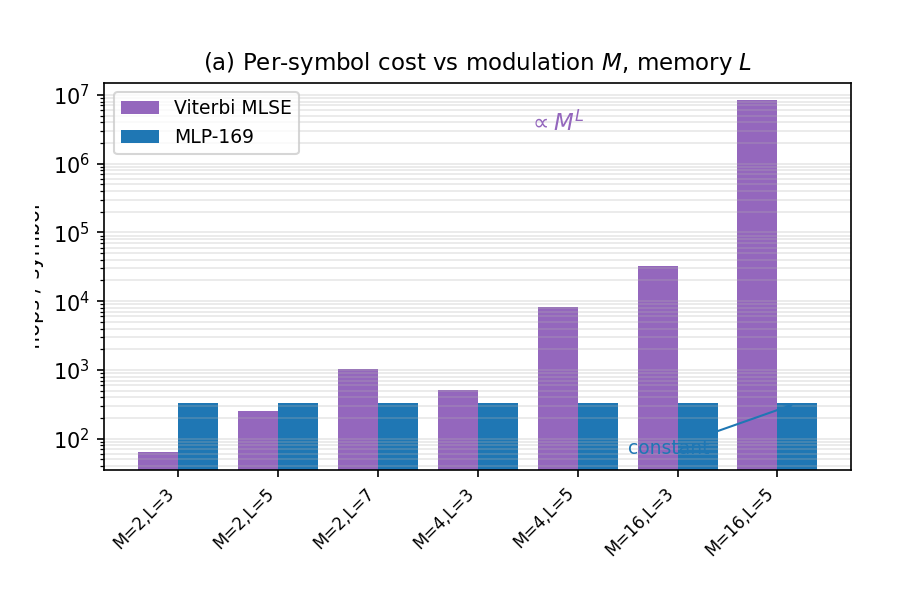
\includegraphics[width=0.8\linewidth]{results/e6_per_symbol_cost_vs_modulation_memory.png}}
\caption{Per-symbol computational cost versus modulation order $M$ and channel memory $L$. Per-symbol operations: Viterbi grows as $M^{L}$ (intractable by $M{=}16,L{=}5$), while the MLP is constant at $\sim$330 flops. On the small studied channel (BPSK, $L{=}3$) Viterbi is actually cheaper; the MLP wins on \emph{scaling}, not on the small case.}
\label{fig:figE6complexity}
\end{figure}

\begin{figure}[H]
\centering
\pandocbounded{
\includegraphics[width=0.8\linewidth]{results/e6_right_clean.png}}
\caption{Measured inference time for BPSK with $L=3$: the MLP is $30$--$90\times$ faster as a vectorized matmul versus Viterbi's interpreted sequential trellis scan.}
\label{fig:e6_inference_time}
\end{figure}
